\documentclass[11pt,a4paper]{article}
\usepackage{amsmath,amssymb,amsthm}
\usepackage{booktabs}
\usepackage{graphicx,float}
\usepackage{geometry}
\usepackage{microtype}
\usepackage{needspace}
\usepackage{listings}
\usepackage{xcolor}
\usepackage{hyperref}
\hypersetup{colorlinks=true, linkcolor=blue, citecolor=blue}
\geometry{margin=1in}
\lstset{basicstyle=\ttfamily\small, frame=single, breaklines=true}

\title{\textbf{Empirical Analysis of Gradient Propagation Dynamics Across Varying Network Depths in GB-Net}}
\author{GB-Net (\texttt{gb\_net\_lib}) --- Experiment 2}
\date{\today}

\begin{document}

\maketitle

\begin{abstract}
\noindent We empirically analyze how gradient signals scale across deep multi-layer perceptrons built with \texttt{gb\_net\_lib}'s \texttt{net} module. Single forward-backward passes are executed at initialization across network depths $L \in \{2, 5, 10, 15, 20\}$ with constant width $N = H = 8$, over seeds $\{0, 1, 42\}$, for three regimes: Sigmoid (\texttt{act='sg'}, squared loss), default ReLU (\texttt{act='relu'}, $\mathcal{U}(-0.5, 0.5)$ initialization), and He-initialized ReLU ($\mathcal{U}(-\sqrt{6/8}, \sqrt{6/8}) \approx \mathcal{U}(-0.866, 0.866)$). We measure the layer-wise weight-gradient Frobenius norm $G_W^{(\ell)} = \|\nabla_{W^{(\ell)}}\mathcal{L}\|_F$, the bias-gradient norm $G_b^{(\ell)}$, the ReLU active-neuron fraction, the end-to-end attenuation ratio $\rho_L = G_W^{(1)}/(G_W^{(L)} + 10^{-30})$, and the per-layer log-decay $\alpha_L = \log_{10}(\rho_L)/(L-1)$. Results are aggregated as mean $\pm$ standard deviation across the three seeds. Sigmoid gradients vanish rapidly: at $L=20$, $\rho_{20} = 8.23 \times 10^{-15}$ ($\alpha \approx -0.74$ dex/layer), leaving early layers effectively untrained. Default ReLU decays more slowly ($\rho_{20} = 6.48 \times 10^{-6}$, $\alpha \approx -0.28$ dex/layer) but still vanishes under $\mathcal{U}(-0.5, 0.5)$ because its weight standard deviation ($0.289$) is below the variance-preserving He value ($0.500$). He-initialized ReLU preserves gradient magnitude ($\rho_{20} \approx 1.25$, $\alpha \approx +0.004$ dex/layer), confirming that variance-scaled initialization mitigates vanishing gradients in this engine.
\end{abstract}

\section{Introduction \& Architectural Overview}

GB-Net's \texttt{net} class constructs an MLP from \texttt{bp} autograd nodes using column vectors. Each layer computes $z^{(\ell)} = W^{(\ell)} h^{(\ell-1)} + b^{(\ell)}$ followed by an activation $\phi^{(\ell)}$, with $W^{(\ell)} \in \mathbb{R}^{n_\ell \times n_{\ell-1}}$ and $b^{(\ell)} \in \mathbb{R}^{n_\ell \times 1}$, and $h^{(0)} = x$. By default, weights and biases are drawn i.i.d. from $\mathcal{U}(-0.5, 0.5)$. Backpropagation through $L$ layers applies the chain rule recursively, so the gradient reaching the first layer is a product of $L-1$ layer Jacobians. Experiment 2 measures how this product scales with depth for different activations and initializations, using a single forward-backward pass per configuration (no training loops), which isolates the structural Jacobian properties at initialization.

\section{Mathematical Formulation}

For an $L$-layer MLP with scalar loss $\mathcal{L}$, forward propagation gives
\[
z^{(\ell)} = W^{(\ell)} h^{(\ell-1)} + b^{(\ell)},
\qquad
h^{(\ell)} = \phi^{(\ell)}\!\left(z^{(\ell)}\right),
\qquad
h^{(0)} = x .
\]
Define the pre-activation sensitivity $\delta^{(\ell)} = \partial\mathcal{L}/\partial z^{(\ell)}$. At the output layer ($h^{(L)} \equiv o$), with squared-error loss defined below,
\[
\delta^{(L)} = \phi'\!\left(z^{(L)}\right) \odot \frac{\partial\mathcal{L}}{\partial h^{(L)}} .
\]
For hidden layers the sensitivity recurses as
\[
\frac{\partial\mathcal{L}}{\partial h^{(\ell)}} = \left(W^{(\ell+1)}\right)^\top \delta^{(\ell+1)},
\qquad
\delta^{(\ell)} = \phi'\!\left(z^{(\ell)}\right) \odot \frac{\partial\mathcal{L}}{\partial h^{(\ell)}} .
\]
Equivalently, collapsing the recurrence, the gradient with respect to the first-layer pre-activation relates to the post-activation gradient via
\[
\frac{\partial\mathcal{L}}{\partial z^{(1)}}
=
\operatorname{diag}\!\left(\phi'\!\left(z^{(1)}\right)\right)
\frac{\partial\mathcal{L}}{\partial h^{(1)}} ,
\]
which expands to
\[
\frac{\partial\mathcal{L}}{\partial z^{(1)}}
=
\operatorname{diag}\!\left(\phi'\!\left(z^{(1)}\right)\right)
\left(W^{(2)}\right)^\top
\operatorname{diag}\!\left(\phi'\!\left(z^{(2)}\right)\right)
\cdots
\left(W^{(L)}\right)^\top
\delta^{(L)} .
\]
The layer-wise parameter gradients follow as
\[
\nabla_{W^{(\ell)}}\mathcal{L} = \delta^{(\ell)} \left(h^{(\ell-1)}\right)^\top,
\qquad
\nabla_{b^{(\ell)}}\mathcal{L} = \delta^{(\ell)} .
\]
Hence $G_W^{(\ell)} = \|\nabla_{W^{(\ell)}}\mathcal{L}\|_F$ inherits the multiplicative attenuation of the Jacobian chain, and gradient stability is governed by (i) the activation derivative $\phi'$ and (ii) the weight variance $\operatorname{Var}(W_{ij})$.

\begin{itemize}
\item \textbf{Sigmoid:} $\sigma'(z) = \sigma(z)(1-\sigma(z)) \in (0, 0.25]$, so $|\sigma'| \le 0.25$ creates a severe per-layer contraction.
\item \textbf{ReLU:} $\operatorname{ReLU}'(z) \in \{0,1\}$, with the active-neuron fraction determining signal retention.
\item \textbf{Variance preservation (He):} For ReLU, preserving \emph{forward activation} variance across layers requires $\operatorname{Var}(W) = 2/n_{\ell-1}$ (fan-in), whereas preserving \emph{backpropagated gradient} variance requires $\operatorname{Var}(W) = 2/n_\ell$ (fan-out). These coincide only when $n_\ell = n_{\ell-1}$; here width is constant at $8$, so both give $\operatorname{std}(W) = \sqrt{2/8} = 0.500$, versus $1/\sqrt{12} \approx 0.289$ for $\mathcal{U}(-0.5, 0.5)$ --- below the He value, causing mild contraction even for ReLU.
\end{itemize}

We define the end-to-end attenuation ratio and per-layer decay (orders of magnitude lost per layer) as
\[
\rho_L = \frac{G_W^{(1)}}{G_W^{(L)} + 10^{-30}},
\qquad
\alpha_L = \frac{\log_{10}(\rho_L)}{L-1},
\]
where the $10^{-30}$ guard prevents division by zero. Unless stated otherwise, $\rho_L$ and $\alpha_L$ are reported as mean $\pm$ standard deviation across the three seeds $\{0, 1, 42\}$.

\section{Experimental Methodology \& Setup}

Single-threaded CPU, NumPy \texttt{float64}, seeds $\{0, 1, 42\}$. Depths $L \in \{2, 5, 10, 15, 20\}$, width $N = H = 8$ (\texttt{layers=[8]*L}). Input $x \sim \mathcal{U}(-0.5, 0.5)^{8\times 1}$, target $y = 0.5\,\mathbf{1}_{8\times 1}$. One forward pass and one \texttt{loss.backprop()} per $(L, \text{regime}, \text{seed})$ (45 micro-passes total). Let $o \equiv h^{(L)}$ denote the network output; the scalar loss is the squared error
\[
\mathcal{L} = \sum_{i=1}^{8} \left(h_i^{(L)} - y_i\right)^2
= \left\| h^{(L)} - y \right\|_2^2
= \left\| o - y \right\|_2^2 .
\]

\needspace{5\baselineskip}
\textbf{Regimes:}
\begin{enumerate}
\item \textbf{Sigmoid:} \texttt{act='sg'}, default $\mathcal{U}(-0.5, 0.5)$ init.
\item \textbf{ReLU (default):} \texttt{act='relu'}, default $\mathcal{U}(-0.5, 0.5)$ init.
\item \textbf{ReLU (He):} \texttt{act='relu'}, weights rescaled to $\mathcal{U}(-\sqrt{6/8}, \sqrt{6/8})$, biases zeroed.
\end{enumerate}

Metrics per layer $\ell$: $G_W^{(\ell)}$ (Frobenius), $G_b^{(\ell)} = \|\nabla_{b^{(\ell)}}\mathcal{L}\|_2$ (Euclidean), and for ReLU the active-neuron fraction $\text{ANF}^{(\ell)} = H^{-1}\sum_i \mathbb{I}(h_i^{(\ell)} > 0)$. Network summary: $\rho_L$, $\alpha_L$. All results are aggregated across 3 seeds (mean $\pm$ std); the CSV in \texttt{RESULTS/exp2/} contains the per-seed values.

\section{Empirical Results \& Analysis}

\subsection{Attenuation across depth}
Table~\ref{tab:rho} reports $\rho_L$ and $\alpha_L$ aggregated over the three seeds. Sigmoid loses roughly $0.73$--$0.79$ orders of magnitude per layer: by $L=20$, $\rho_{20} = 8.23 \times 10^{-15}$, i.e. the first-layer gradient is 14 orders below the output-layer gradient. Default ReLU decays more slowly but still vanishes ($\rho_{20} = 6.48 \times 10^{-6}$, $\alpha \approx -0.28$ dex/layer). He-initialized ReLU preserves magnitude ($\rho_{20} \approx 1.25$, $\alpha \approx +0.004$ dex/layer).

\begin{table}[H]
\centering
\caption{Attenuation ratio $\rho_L$ and per-layer decay $\alpha_L$, mean $\pm$ std over seeds $\{0,1,42\}$. $G_W$ columns show the mean across seeds.}
\label{tab:rho}
{\small
\setlength{\tabcolsep}{4pt}
\begin{tabular}{lcccccc}
\toprule
Activation & $L$ & mean $G_W^{(1)}$ & mean $G_W^{(L)}$ & $\rho_L$ & $\alpha_L$ \\
\midrule
Sigmoid & 2  & $2.86\times10^{-2}$ & $1.71\times10^{-1}$ & $1.65\times10^{-1} \pm 1.50\times10^{-2}$ & $-0.784 \pm 0.040$ \\
Sigmoid & 5  & $1.82\times10^{-4}$ & $2.35\times10^{-1}$ & $7.57\times10^{-4} \pm 2.64\times10^{-4}$ & $-0.787 \pm 0.037$ \\
Sigmoid & 10 & $3.03\times10^{-8}$ & $1.91\times10^{-1}$ & $1.59\times10^{-7} \pm 6.39\times10^{-8}$ & $-0.761 \pm 0.025$ \\
Sigmoid & 15 & $7.17\times10^{-12}$ & $1.86\times10^{-1}$ & $3.72\times10^{-11} \pm 9.78\times10^{-12}$ & $-0.746 \pm 0.008$ \\
Sigmoid & 20 & $2.11\times10^{-15}$ & $2.60\times10^{-1}$ & $8.23\times10^{-15} \pm 3.40\times10^{-15}$ & $-0.743 \pm 0.010$ \\
ReLU (default) & 2  & $6.39\times10^{-1}$ & $8.54\times10^{-1}$ & $7.19\times10^{-1} \pm 7.69\times10^{-2}$ & $-0.146 \pm 0.045$ \\
ReLU (default) & 5  & $1.32\times10^{-1}$ & $1.06\times10^{0}$ & $9.70\times10^{-2} \pm 4.38\times10^{-2}$ & $-0.263 \pm 0.045$ \\
ReLU (default) & 10 & $5.74\times10^{-3}$ & $5.15\times10^{-1}$ & $1.11\times10^{-2} \pm 1.63\times10^{-3}$ & $-0.218 \pm 0.007$ \\
ReLU (default) & 15 & $2.53\times10^{-4}$ & $7.28\times10^{-1}$ & $3.29\times10^{-4} \pm 3.72\times10^{-4}$ & $-0.300 \pm 0.078$ \\
ReLU (default) & 20 & $5.41\times10^{-6}$ & $8.21\times10^{-1}$ & $6.48\times10^{-6} \pm 3.22\times10^{-6}$ & $-0.277 \pm 0.013$ \\
ReLU (He) & 2  & $1.06\times10^{0}$ & $1.14\times10^{0}$ & $9.34\times10^{-1} \pm 7.73\times10^{-2}$ & $-0.031 \pm 0.035$ \\
ReLU (He) & 5  & $1.37\times10^{0}$ & $6.10\times10^{-1}$ & $4.13\times10^{0} \pm 4.00\times10^{0}$ & $+0.088 \pm 0.128$ \\
ReLU (He) & 10 & $1.05\times10^{0}$ & $9.62\times10^{-1}$ & $1.06\times10^{0} \pm 1.60\times10^{-1}$ & $+0.002 \pm 0.007$ \\
ReLU (He) & 15 & $3.42\times10^{-1}$ & $2.04\times10^{-1}$ & $1.67\times10^{0} \pm 2.83\times10^{-1}$ & $+0.015 \pm 0.006$ \\
ReLU (He) & 20 & $3.97\times10^{-1}$ & $2.65\times10^{-1}$ & $1.25\times10^{0} \pm 4.44\times10^{-1}$ & $+0.004 \pm 0.008$ \\
\bottomrule
\end{tabular}}
\end{table}

Figure~\ref{fig:decay} (Panel A) plots 3-seed mean $\log_{10}\rho_L$ vs. $L$; Panel B shows the layer-by-layer profile $\log_{10}G_W^{(\ell)}$ at $L=20$ (seed 42).

\begin{figure}[H]
\centering
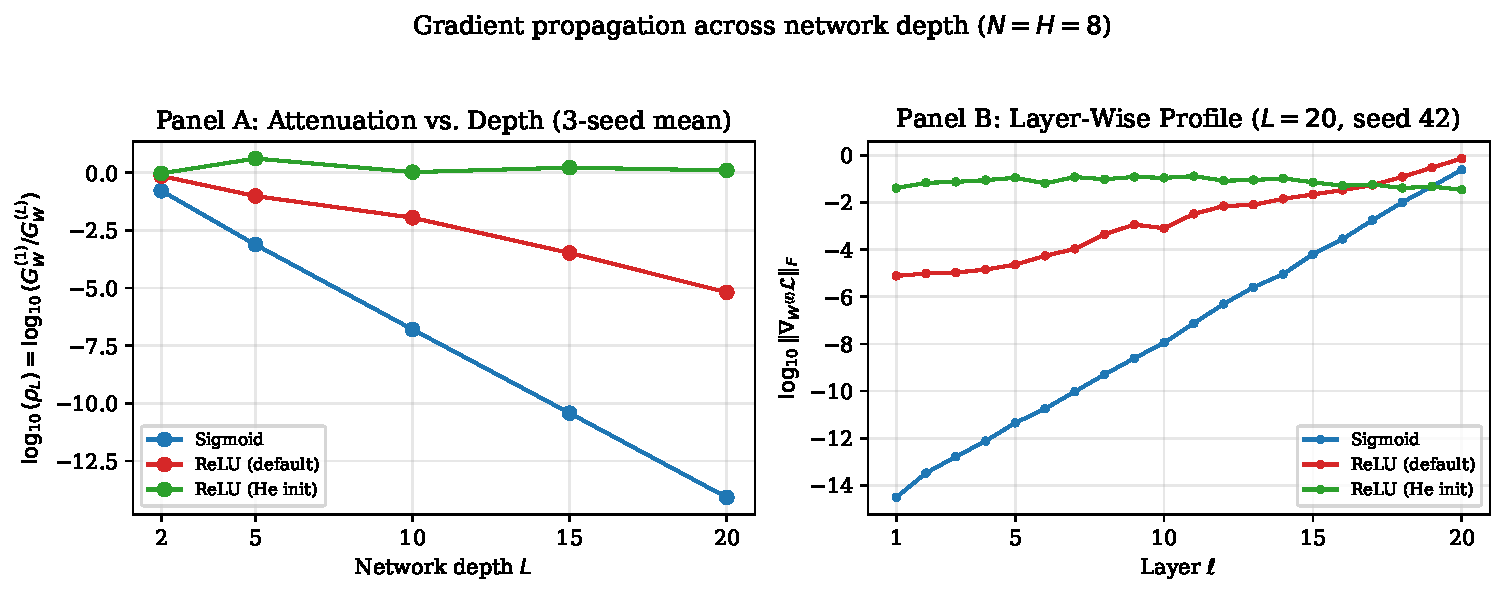
\includegraphics[width=1.0\linewidth]{../../RESULTS/exp2/fig3_depth_decay_comparison.pdf}
\caption{Gradient attenuation vs. depth (Panel A: 3-seed mean) and layer-wise profile at $L=20$ (Panel B: seed 42).}
\label{fig:decay}
\end{figure}

\subsection{Layer-wise profile and bias gradients}
At $L=20$, the Sigmoid profile shows steep monotonic decay from the output layer back to the input (roughly linear on the log scale, slope $-0.743 \pm 0.010$ dex/layer), so the first layer's gradient is numerically zero for practical learning rates: \texttt{w.data -= lr * w.grad} applies a numerically zero update to $W^{(1)}$. Default ReLU shows a shallower decay. He-initialized ReLU shows an essentially flat profile ($\alpha \approx 0$), confirming that variance-scaled initialization counteracts the contraction of the Jacobian chain.

Table~\ref{tab:bias} reports the bias-gradient norm $G_b^{(\ell)}$ and ReLU active-neuron fraction at $L=20$ for representative layers. Both columns report 3-seed means (each ANF value is an average over $3 \times 8 = 24$ neuron-seed combinations). Bias gradients mirror the weight-gradient decay: Sigmoid $G_b^{(1)} \approx 2.45 \times 10^{-15}$ (vanished), while He-ReLU retains $G_b^{(1)} \approx 4.96 \times 10^{-1}$. The active-neuron fraction stays far below one for ReLU ($\approx 0.3$--$0.55$), indicating that a substantial fraction of ReLU units are inactive at initialization and contribute no gradient signal.

\begin{table}[H]
\centering
\caption{Bias-gradient norm $G_b^{(\ell)}$ and active-neuron fraction $\text{ANF}^{(\ell)}$ at $L=20$, 3-seed means.}
\label{tab:bias}
{\small
\setlength{\tabcolsep}{5pt}
\begin{tabular}{lcccccc}
\toprule
Layer $\ell$ & \multicolumn{2}{c}{Sigmoid} & \multicolumn{2}{c}{ReLU (default)} & \multicolumn{2}{c}{ReLU (He)} \\
 & $G_b$ & ANF & $G_b$ & ANF & $G_b$ & ANF \\
\midrule
1  & $2.45\times10^{-15}$ & 1.000 & $5.97\times10^{-6}$ & 0.458 & $4.96\times10^{-1}$ & 0.292 \\
5  & $1.93\times10^{-12}$ & 1.000 & $6.34\times10^{-5}$ & 0.417 & $5.73\times10^{-1}$ & 0.375 \\
10 & $9.34\times10^{-9}$ & 1.000 & $1.95\times10^{-3}$ & 0.500 & $1.46\times10^{0}$ & 0.542 \\
15 & $3.43\times10^{-5}$ & 1.000 & $5.95\times10^{-2}$ & 0.542 & $1.14\times10^{0}$ & 0.458 \\
20 & $1.65\times10^{-1}$ & 1.000 & $1.06\times10^{0}$ & 0.542 & $1.21\times10^{0}$ & 0.333 \\
\bottomrule
\end{tabular}}
\end{table}

\subsection{Per-seed variability}
The standard deviations in Table~\ref{tab:rho} are small relative to the mean for Sigmoid and default ReLU (e.g. Sigmoid $L=20$: $\alpha = -0.743 \pm 0.010$), confirming that the vanishing-gradient trend is a structural property of the Jacobian chain rather than seed-dependent noise. He-ReLU shows larger relative scatter at small depth ($L=5$: $\alpha = +0.088 \pm 0.128$) because $\rho_5$ is sensitive to the random realization of the rescaled weights, but by $L=20$ it stabilizes ($\alpha = +0.004 \pm 0.008$).

\section{Architectural Discussion \& Conclusion}

Experiment 2 confirms the classical vanishing-gradient mechanism in GB-Net: backpropagating through $L$ layers multiplies $L-1$ matrices $(W^{(\ell)})^\top \operatorname{diag}(\phi'(z^{(\ell)}))$, so gradient magnitude at the first layer is exponentially sensitive to the activation derivative and weight variance. Sigmoid's bounded derivative ($\le 0.25$) causes rapid vanishing ($\alpha \approx -0.75$ dex/layer), rendering $W^{(1)}$ untrainable at depth by $L=20$. ReLU mitigates but does not eliminate the problem under \texttt{gb\_net\_lib}'s fixed $\mathcal{U}(-0.5, 0.5)$ initialization: with width 8, the He-preserving standard deviation is $0.500$ versus $0.289$ actually used, producing mild per-layer contraction ($\alpha = -0.277 \pm 0.013$, i.e. $\approx -0.28$ dex/layer). He-scaled uniform initialization ($\operatorname{std}=0.500$, zero biases) restores gradient preservation ($\rho_{20} \approx 1.25$).

Concrete recommendations:
\begin{enumerate}
\item Adopt He/Xavier variance-scaled initialization for ReLU/Sigmoid networks (matching fan-in for forward variance and fan-out for gradient variance).
\item Consider bias initialization and activation scaling to keep pre-activations away from saturation.
\item Insert normalization layers (e.g., LayerNorm) and/or residual connections, which rescale activations and gradients and thereby preserve signal magnitude to early layers.
\end{enumerate}

The single-pass, no-training design keeps runtime well under the sub-second budget while isolating the structural Jacobian behavior at initialization.

\end{document}
